\documentclass[10pt]{article}

% --- Page geometry (NeurIPS-style) ---
\usepackage[letterpaper,left=1.5in,right=1.5in,top=1in,bottom=1in]{geometry}

% --- Fonts: Times-like ---
\usepackage[T1]{fontenc}
\usepackage[utf8]{inputenc}
\usepackage{newtxtext}
\usepackage{microtype}

% --- Math and tables ---
\usepackage{amsmath,amsfonts,mathtools,amsthm}
\usepackage{newtxmath}
\newtheorem{proposition}{Proposition}
\newtheorem{theorem}{Theorem}
\newtheorem{corollary}{Corollary}
\usepackage{booktabs}
\usepackage{longtable}
\usepackage{array}
\usepackage{tabularx}

% --- Lists ---
\usepackage{enumitem}
\setlist[itemize]{leftmargin=1.5em, itemsep=2pt, topsep=4pt, parsep=0pt}
\setlist[enumerate]{leftmargin=1.6em, itemsep=2pt, topsep=4pt, parsep=0pt}

% --- Colors, graphics, links ---
\usepackage{xcolor}
\usepackage{graphicx}
\usepackage{xurl}
\usepackage[hidelinks,unicode]{hyperref}

% --- TikZ and figures ---
\usepackage{tikz}
\usepackage{pgfplots}
\pgfplotsset{compat=1.18}
\usetikzlibrary{arrows.meta,positioning,calc,patterns,decorations.pathreplacing,shapes.geometric}
\usepackage[font=small, labelfont=bf, labelsep=period]{caption}
\graphicspath{{figures/}}

% --- Paragraph and spacing ---
\setlength{\parindent}{0pt}
\setlength{\parskip}{5.5pt}
\setlength{\emergencystretch}{2em}
\frenchspacing

\urlstyle{same}
\hypersetup{
  pdftitle={Trust-Explicit Resolution for Prediction Markets},
  pdfauthor={Andrei Savin}
}

\setcounter{tocdepth}{2}
\setcounter{secnumdepth}{2}

% --- Section formatting (NeurIPS-style) ---
\usepackage{titlesec}
\titleformat{\section}{\normalfont\large\bfseries}{\thesection}{0.6em}{}
\titleformat{\subsection}{\normalfont\normalsize\bfseries}{\thesubsection}{0.6em}{}
\titleformat{\subsubsection}{\normalfont\normalsize\itshape}{\thesubsubsection}{0.5em}{}
\titlespacing*{\section}{0pt}{10pt plus 2pt minus 2pt}{4pt plus 1pt minus 1pt}
\titlespacing*{\subsection}{0pt}{8pt plus 2pt minus 2pt}{3pt plus 1pt minus 1pt}
\titlespacing*{\subsubsection}{0pt}{6pt plus 2pt minus 1pt}{2pt plus 1pt minus 1pt}

% --- Page style: just page numbers ---
\pagestyle{plain}

% --- Abstract environment (NeurIPS-style) ---
\renewenvironment{abstract}{%
  \centerline{\bfseries\normalsize Abstract}%
  \vspace{0.5ex}%
  \begin{quote}\small
}{%
  \end{quote}%
}

% --- Helpers ---
\newcolumntype{Y}{>{\raggedright\arraybackslash}X}

\newcommand{\artifactfigure}[3]{%
  \begin{figure}[t]
  \centering
  \IfFileExists{#1}{%
    \includegraphics[width=#2\linewidth]{#1}%
  }{%
    \fbox{%
      \parbox{0.8\linewidth}{%
        \small Figure asset not found at build time: \texttt{#1}%
      }%
    }%
  }
  \caption{#3}
  \end{figure}
}

\begin{document}

\begin{center}
{\LARGE\bfseries Trust-Explicit Resolution for Prediction Markets\par}
\vspace{0.4em}
{\large Declared Logic, Verifiable Traces, and Dispute Economics\par}
\vspace{1.2em}
{\normalsize\bfseries Andrei Savin\par}
\vspace{0.3em}
{\small question.market\par}
{\small\href{mailto:andrei@andreisavin.com}{andrei@andreisavin.com}\par}
\vspace{0.6em}
{\small April 2026; revised October 2026\par}
\end{center}

\vspace{0.8em}

\begin{abstract}

Prediction markets put money behind beliefs, but their value depends on resolution: the process that decides which outcome occurred and who gets paid. Publishing a question and naming an oracle leaves much of that process outside the market's executable rules. Participants are also betting on how evidence and ambiguity will be interpreted when money has to move.

This paper develops \emph{trust-explicit} resolution. Each market commits an immutable executable constitution: a typed resolution blueprint specifying evidence sources, judgment steps, routing, deadlines, cancellation, and dispute rules. A derived trust profile exposes its authorities and verification boundaries. Canonical full-trace commitments, source authentication, independent replay, and a publication deadline turn the declared procedure into a challengeable execution record.

The economic thesis is direct. Flat bonds fail as extractable exposure grows while correction remains imperfect. Thin-market integrity is constrained by actual checking, not just adjudicator sophistication. Open proposal and verification work must be funded. We prove a bond--coverage deterrence frontier, the failure of sublinear exposure penalties, the rare-fraud constraint of bounty-only inspection, and sufficient conditions for a funded truthful-inspection equilibrium in which checking beats shirking. We also prove the corruption threshold of composed sources and show how shared authorities collapse it.

The evidence consists of 855{,}000 funded-game episodes, exact inspection equilibria checked by 900{,}000 Monte Carlo episodes, and an executable authenticated-blueprint prototype with exhaustive source-state tests and adversarial trace tests. In a low-attention market, proportional bonds reduce wrong outcomes substantially but do not replace coverage. Paid auditable inspection can sustain truthful resolution. A construction without extra work collateral preserves challenge capacity, while unaudited retainers buy shirking. Executed two-of-three source composition reduces independent 5\% source error to 0.725\%, while a matched-marginal common-error control exposes the cost of dependence. These results yield a concrete protocol: commit the resolution constitution, fund its execution and checking, and size its economic guarantees against measured exposure and correction capacity.

\end{abstract}

\vspace{1em}
{
\small
\renewcommand{\contentsname}{}
\setcounter{tocdepth}{2}
\tableofcontents
}
\vspace{0.5em}

\section{Introduction}

Prediction markets work because participants risk capital on outcomes. A share in ``Team A wins'' that pays \$1 if correct and \$0 otherwise carries economic consequence for the buyer. That consequence is what separates a prediction market from a poll. It is also why resolution, the process that determines which shares pay out, is the most important part of the system. Everything else (pricing, liquidity, order matching) is infrastructure. Resolution is where participants' money actually changes hands.

This would be unremarkable if resolution were a solved problem. It is not. In Polymarket, resolution works as follows: the platform team defines the question, an external oracle system (UMA's Optimistic Oracle) accepts bonded proposals, and if nobody disputes within a window, the proposal finalizes \cite{uma2021}. The mechanism has useful properties: it is bonded, it is challengeable, and it has an escalation path. But the part participants are actually betting on is still drafted and interpreted through a platform-authored specification rather than an immutable executable workflow committed by the market itself. The bonded assertion fixes an answer and an escalation route; a market-native program can additionally fix how evidence is gathered and transformed into that answer.

Other systems make different tradeoffs. Reality.eth provides a bonded-answer primitive where anyone can propose an answer, subsequent proposals require larger bonds, and disputes can escalate to a configured external arbitrator, including Kleros \cite{realityeth}. The mechanism is more decentralized than a platform-controlled oracle, but the resolution logic is external to the market: the market references an oracle contract but does not itself declare how truth will be determined. Centralized platforms resolve by editorial discretion, which is the fastest and cheapest approach and also the one that provides the least structural accountability.

The thesis of this paper is that a stronger property is achievable and worth pursuing. We call it \emph{trust-explicit} resolution. Every prediction market resolution system depends on some external input about what actually happened in the world. The design goal is therefore not to remove trust, but to bind it to declared procedures that participants can inspect before trading and challenge after execution. Markets should commit to an executable decision program, not just to a question string or an oracle brand. A system that declares that program at market creation, stores it immutably, executes it to produce a verifiable trace, and backs the result with bonded dispute economics makes more of the resolution process declared, inspectable, and challengeable up front.

The contribution has three parts. Section~\ref{sec:stratification} defines a trust stratification framework with five properties and maps existing systems to it. Sections~\ref{sec:blueprints} and~\ref{sec:trustclasses} describe the resolution blueprint mechanism: a typed DAG with a minimal step vocabulary, automatic trust classification, and immutable on-chain commitment. Section~\ref{sec:dispute} presents the paper's main analytical contribution: a game-theoretic model of dispute economics that derives bond sizing requirements, identifies the lazy verifier problem, and analyzes challenge-linked verifier incentives. Section~\ref{sec:simulation} describes an agent-based simulation program that tests the analytical results across market conditions. Section~\ref{sec:results} presents findings.

This contribution is orthogonal to the trading mechanism. LMSR-style automated market makers \cite{hanson2002}, order-book exchange designs, and conditional-token architectures can each support trading, but none of them by themselves answer the resolution question. Conditional tokens, for example, already formalize a condition as ``a question to be answered in the future by a specific oracle'' \cite{gnosisct2026}; the blueprint proposal extends that idea from a single oracle hook to an executable and challengeable resolution program.

\subsection{What is new here}

Disputes, optimistic oracles, and arbitration backstops are already part of the deployed ecosystem. Systems such as Polymarket/UMA and Reality.eth/Kleros already show that bonded proposals, challenge windows, and escalation can work in production. The contribution is the integration of executable market rules, an explicit trust profile, and funded resolution economics.

Three pieces matter:
\begin{enumerate}
\item \textbf{Blueprint formalism.} A blueprint binds evidence acquisition, interpretation, routing, cancellation, and the dispute path to the individual market before any answer is proposed.
\item \textbf{Trust semantics.} The trust class/profile vocabulary turns the resolution trust surface into protocol-visible state rather than leaving it embedded in natural-language norms.
\item \textbf{Resolution economics.} The paper treats resolution as its own mechanism-design problem, with the lazy-verifier problem and bond scaling as primary constraints rather than as operational details downstream of trading.
\end{enumerate}

Declared logic, verifiable traces, and funded dispute economics turn resolution from an oracle label into an inspectable mechanism. The contribution is constructive: a language and verifier, proofs of their commitment and incentive properties, and experiments that execute the attacks those proofs distinguish.

\subsection{Related work}

This paper connects prediction-market resolution, programmable oracles, and verification games.

\textbf{Bonded resolution and arbitration.} UMA exposes bonded proposals, rewards for accepted proposals, a challenge period, and escalation to its Data Verification Mechanism \cite{uma2021}. Reality.eth combines successively bonded answers with a configurable arbitration backstop, commonly Kleros \cite{realityeth,kleros2019}. Augur and Schelling-point designs address agreement over disputed external facts \cite{augurv2,buterin2014,sztorc2015}. Proposer rewards and economic disputes are established mechanisms. This paper derives their participation and deterrence conditions together with the cost of checking a declared resolution program.

\textbf{Programmable oracle requests.} Witnet already specifies executable requests with multiple sources, extraction, filtering, aggregation, and tallying, compiled into request bytecode \cite{witnet2026}. Executable source processing and source composition therefore have clear prior art. Conditional Tokens also permit a question identifier to reference richer off-chain material; their core contract defines oracle-addressed payout conditions rather than prescribing how an oracle reasons \cite{gnosisct2026}. The blueprint contribution is a market-level constitution that joins source processing to judgment steps, explicit defer/cancel behavior, a fixed dispute path, an automatically derived trust profile, and a funded inspection game. It can use such oracle infrastructure as a component.

\textbf{Oracle security.} Chainlink formalizes decentralized oracle networks \cite{chainlink2017}; Eskandari et al.\ systematize oracle trust and manipulation risks \cite{eskandari2021}. Our source-corruption experiments instantiate those risks inside executable event-resolution workflows. Distinct endpoints need not be independent authorities. Source authenticity, data availability, executor integrity, and semantic truth are separate attack surfaces.

\textbf{The verifier's dilemma.} TrueBit studies how costly checking can sustain a verification game when errors are rare \cite{teutsch2019}. Koch and Reitwie\ss ner propose more predictable compensation through selected solvers and shared fees \cite{koch2018}. We specialize this problem to prediction-market resolution, where a participant's outcome exposure can motivate either honest correction or false challenge, and derive a verify/shirk/idle equilibrium. Our paid-inspection construction states the audit condition that makes actual checking privately preferable to collecting a retainer without doing the work.

\textbf{Trading and external incentives.} Trading designs such as LMSR \cite{hanson2002} are orthogonal to resolution. The MEV literature \cite{daian2019} underscores why a bond must cover the attacker's gain, including connected positions when they exist. Pool collateral bounds the funded single-market claims in our experiments; it cannot bound an attacker's entire external portfolio.

\section{Why Resolution Is the Hard Problem}

\subsection{What participants need to know}

Before placing a trade, a rational participant in a prediction market needs four pieces of information about the resolution process:

\begin{enumerate}
\item \textbf{What} will determine the outcome. Is it an API data feed, a human judgment, an AI evaluation, or some combination?
\item \textbf{Who} will execute the determination. Is it the platform, a designated oracle, any willing party, or an automated process?
\item \textbf{What happens if the determination is wrong.} Is there a dispute mechanism? What does it cost to trigger? Who adjudicates?
\item \textbf{What recourse exists.} If the dispute mechanism itself fails, what is the fallback?
\end{enumerate}

Most deployed prediction markets answer some of these questions, but usually in a scattered way: part in market text, part in docs, part in oracle policy, part in community norms. A participant still has to piece the resolution surface together from multiple places. The result is structural opacity: the information may exist, but it is rarely exposed in a single market-native form that can be inspected, compared, or enforced at the protocol level.

\subsection{Resolution in deployed systems}

Three common resolution architectures illustrate the design space.

\textbf{Platform-controlled resolution.} A centralized team drafts the question, interprets the outcome, and resolves the market. This is fast, cheap, and administratively simple. The failure mode is discretionary risk: the same team that benefits from market activity controls the resolution. Even without bad intent, interpretation of ambiguous outcomes introduces inconsistency that participants cannot predict or challenge structurally.

\textbf{Oracle-delegated resolution.} The market delegates resolution to an external oracle contract. UMA's Optimistic Oracle, used by Polymarket, is the most prominent example \cite{uma2021}. A proposer bonds a claim about the outcome; if nobody disputes within a window, the claim finalizes. Disputes escalate to UMA token-holder voting. The mechanism provides economic accountability when false proposals are challenged and rejected. But the market's question specification is still controlled by the platform, and the oracle's interpretation of that specification is a separate trust assumption layered on top.

\textbf{Bonded-answer escalation.} Reality.eth allows anyone to propose an answer to a question, with each subsequent proposal requiring a higher bond \cite{realityeth}. If no higher-bonded counter-proposal arrives within the timeout, the last answer wins. A configured arbitrator can settle disputes; Kleros is a common choice \cite{kleros2019}. This is one of the more decentralized resolution approaches in production. The resolution logic, however, is external to the market. A market on Seer references a Reality.eth question, but the market itself does not declare how the answer will be determined. The resolution specification is a natural-language question string, not a structured program.

The distinction is easiest to see at market creation time: what exactly becomes immutable before trading begins?

\begin{table}[t]
\centering
\caption{The object a participant can inspect. These are architectural distinctions; an integration can combine them.}
\label{tab:creation_commitment}
\small
\begin{tabularx}{\linewidth}{@{}p{0.24\linewidth}YY@{}}
\toprule
Architecture & Declared object & Remaining decision surface \\
\midrule
Platform resolution & Market rules and editorial policy & Interpretation and the platform's change policy \\
Optimistic assertion & Question, bonded answer, dispute rules & Evidence-to-answer procedure unless separately specified \\
Bonded-answer oracle & Question, answer game, arbitrator & External interpretation of the question \\
Programmable oracle & Source query, extraction and aggregation & Market-specific judgment and fallback policy \\
Blueprint market & Versioned main/dispute programs and trust profile & Declared external inputs and adjudication authority \\
\bottomrule
\end{tabularx}
\end{table}

Operational experience makes the distinction concrete. In August 2025 UMA introduced managed proposers: integrations could configure a proposer whitelist while disputes remained permissionless. UMA's stated motivations were low-quality or premature proposals and the resulting operational overhead \cite{umamoop2025}. That episode demonstrates that permission to propose, quality of proposing, and availability of challenges are separate design variables. It does not identify unpaid work as the cause: UMA already supports proposer rewards. The participation model below establishes the compensation requirement directly.

Polymarket's published resolution guide describes predefined market rules, a bonded proposal, a reward for an accepted proposal, and a two-hour challenge period \cite{polymarket2024}. The economic question is what coverage that period buys for a particular market. A clock is not a checker. The analysis below therefore derives a window from measured checker arrival and a target correction probability, rather than inferring security from the advertised duration.

\subsection{Failure taxonomy}
\label{sec:failures}

Resolution failures are not all the same. Six distinct failure modes affect prediction market resolution:

\begin{center}
\setlength{\LTleft}{0pt}
\setlength{\LTright}{0pt}
\setlength{\tabcolsep}{4pt}
\renewcommand{\arraystretch}{1.15}
\footnotesize
\begin{longtable}{@{}>{\raggedright\arraybackslash}p{0.22\linewidth} >{\raggedright\arraybackslash}p{0.34\linewidth} >{\raggedright\arraybackslash}p{0.30\linewidth}@{}}
\toprule
Failure Mode & Description & Primary Exposure \\
\midrule
\endfirsthead
\toprule
Failure Mode & Description & Primary Exposure \\
\midrule
\endhead
Ambiguous specification & The question admits multiple valid interpretations & All systems using natural-language questions \\
Interpretive discretion & The resolver chooses one interpretation without structural accountability & Platform-controlled resolution \\
Data source failure & The oracle or API that provides ground truth is down, wrong, or manipulated & Oracle-delegated and bonded-answer systems \\
Executor malfeasance & The party executing the resolution submits a deliberately false outcome & Any system with a single resolution executor \\
Liveness failure & Nobody submits or checks a valid resolution & Designated and permissionless resolver systems \\
Escalation capture & The dispute adjudicator is compromised or colluding with one party & Any delegated adjudication authority \\
\bottomrule
\end{longtable}
\end{center}
\normalsize
\setlength{\tabcolsep}{6pt}

No single system is immune to all six. The relevant question is not ``which system eliminates all failure modes'' but ``which system makes its failure exposures visible and provides structural countermeasures for the most dangerous ones.''

Question quality sits upstream of every dispute game. Forecasting platforms with strong editorial discipline explicitly require authoritative sources, explicit edge-case handling, and fallback criteria in their resolution text \cite{metaculus2026}. A blueprint cannot rescue a malformed or semantically incoherent market specification. The relevant design object is therefore the pair \emph{(question specification, blueprint)}, not the blueprint in isolation. In practice that means the question side should also become more structured over time: typed outcome domains, explicit temporal scope, declared tie-breaking rules, named fallback-to-cancel conditions, and stated handling for foreseeable edge cases. Blueprint authoring quality belongs in the same upstream threat model. Stronger declaration makes bad logic legible, but it also makes that logic immutable once trading begins. Compiler and runtime validation can reject malformed programs; they cannot guarantee that a declared workflow is economically sensible, semantically fair, or robust to adversarial wording.

\section{Trust Stratification}
\label{sec:stratification}

Trust explicitness has five dimensions: declaredness, inspectability, reproducibility, challengeability, and decentralization. They form a profile, not a logical ladder. An immutable but unavailable program is declared and uninspectable. An openly published procedure can be inspectable and mutable. A reproducible computation can faithfully process a false input. Each property answers a different question; combining them is the design objective.

\subsection{Declared}

A market is \emph{declared} when its resolution specification is fixed before trading and cannot be changed while the resulting claims remain outstanding. For market $m$, creation time $t_0$, and full specification $R_m$,
\[
  R_m(t)=R_m(t_0),\qquad t\geq t_0.
\]
The committed object includes the question, outcome domain, program and interpreter version, node parameters, main and dispute paths, deadlines, cancellation rule, source authorities, and permitted upgrade or fallback authority. Fixing a URL while its meaning or interpreter can change is insufficient. A declared upgrade policy is visible authority; it is not immutability of the rules it may replace. Our core construction fixes the rules themselves.

\subsection{Inspectable}

An inspectable market makes the canonical specification retrievable and publishes complete semantics for its language. A reader or tool can determine which authority is consulted at each step and what each possible response permits the program to do. This is an objective interface requirement, not an assertion that every trader can understand every program.

Most participants will consume a rendered workflow, trust class, source list, and warnings. Specialists can inspect the canonical object and reproduce those summaries. This makes program quality visible before money moves. Greater visibility can expose a bad market as readily as a good one; the paper does not assume that transparency mechanically raises willingness to pay. The gain is the ability to condition participation on the actual resolution process.

\subsection{Reproducible, source-verifiable, and trace-verifiable}

Three checks must be distinguished:
\begin{enumerate}
\item \textbf{Replay consistency.} A verifier reproduces routing, extraction, deterministic outputs, and the terminal action from a fixed evidence bundle.
\item \textbf{Source authenticity.} A verifier authenticates an input to the authority named in the blueprint, using a signature or another declared attestation. Archiving unsigned bytes makes them replayable, not authentic.
\item \textbf{Truth or judgment.} A source can sign a false statement; an authorized model or human can make a bad judgment. These disputes require external evidence or the declared adjudication path.
\end{enumerate}

A deterministic trace is fully replayable relative to its inputs. A signed source object is additionally source-verifiable. A live unsigned response or unauthenticated model output supports only inspection of what the executor reported. Full-trace hashing binds that report; it does not promote the report into authenticated evidence. The prototype tests a fabricated, internally consistent trace precisely to enforce this distinction.

\subsection{Challengeable}

A challengeable market exposes a bonded dispute route with a fixed window, evidence requirements, and adjudication rule. Operational challengeability also requires available evidence, a verifier willing to inspect it, and liquid capital to post the challenge bond before the deadline. The economic analysis treats all three explicitly. Declaring a dispute function while making its use infeasible does not produce effective accountability.

\subsection{Decentralized}

Decentralization describes the distribution of authority over execution, sources, arbitration, and finalization. It is not one checkbox. Multiple executors can depend on one source; many signers can share one upstream provider; a public challenge route can end at a concentrated adjudicator. A centralized executor can still be tightly constrained by immutable rules, authentic inputs, independent replay, and effective challenges. These dimensions should be displayed separately so that distributed execution does not conceal concentrated authority.

\subsection{Mapping resolution mechanisms}

\begin{table}[t]
\centering
\caption{Five questions that make trust visible across architectures. The answer is a property of the configured market, not just its oracle's brand.}
\label{tab:stratification}
\small
\begin{tabularx}{\linewidth}{@{}p{0.25\linewidth}Y@{}}
\toprule
Dimension & Inspectable evidence \\
\midrule
Declared & Hash of the full specification; fixed interpreter; change and fallback authorities \\
Inspectable & Available canonical bytes; complete semantics; independently generated summaries \\
Reproducible & Deterministic replay results; source-authentication policy; declared judgment boundary \\
Challengeable & Available trace; funded and capital-eligible checking; usable deadline and adjudication \\
Decentralized & Separate identities and dependencies for sources, executors, auditors, and adjudicators \\
\bottomrule
\end{tabularx}
\end{table}

This framing preserves the important comparison. Natural-language question rules and oracle-addressed claims declare useful information. A blueprint adds an executable account of evidence selection, interpretation, branching, and fallback. Programmable oracle systems already supply parts of that account; the market constitution assembles them with its dispute and funding rules. Trust-explicit resolution makes the entire dependency chain available for inspection.

\section{Resolution Blueprints}
\label{sec:blueprints}

A resolution blueprint is a finite program that defines how a market's question will be answered. The market carries an \emph{executable constitution}: evidence acquisition, interpretation, routing, cancellation, and dispute rules are fixed before trading begins.

\subsection{The committed specification}

The market commits a versioned object $R$ containing the question and outcome domain, a main blueprint, a dispute blueprint, the final fallback, the funding rules, and the interpreter profile. A content-addressed object can carry the bytes off-chain while a contract fixes its identifier before trading. Content addressing binds bytes. A retrieval and publication rule supplies availability. Both are required.

A blueprint is a tuple
\[
G=(V,E,\tau,\theta,\gamma,\beta),
\]
where $V$ is a finite node set, $E$ is a directed \emph{acyclic} edge set, $\tau$ assigns step types, $\theta$ assigns typed node parameters, $\gamma$ assigns Boolean edge guards, and $\beta$ fixes node, byte, time, token, and run budgets. Parameters include source keys, extraction rules, model prompts, judge identities, and terminal outcome mappings. They are part of the commitment, not mutable executor configuration.

Each run is a DAG. Retrying means ending with \texttt{defer\_resolution} and starting a new, numbered run under the committed schedule. There are no back-edges. A new run binds the previous root, starts at its authorized time, and cannot replace a submitted or cancelled run. A finite run cap and market deadline prevent endless deferral.

\subsection{Step vocabulary}

Eight step types define the authoring language. Trust arises at the input and judgment steps; waiting and terminal actions provide control flow.

\begin{center}
\small
\begin{longtable}{@{}p{0.28\linewidth}p{0.65\linewidth}@{}}
\toprule
Type & Committed behavior \\
\midrule
\endfirsthead
\toprule Type & Committed behavior \\
\midrule
\endhead
\texttt{api\_fetch} & Request and extraction rule, source authority, authentication policy, observation cutoff, and missing-data behavior. \\
\texttt{market\_evidence} & Eligible evidence issuers, signatures, ordering, deduplication, submission cutoff, and selection rule. \\
\texttt{llm\_judge} & Provider/model, prompt, parameters, evidence inputs, verdict schema, and response-authentication policy. \\
\texttt{human\_judge} & Judge or panel, rubric, authorized response format, quorum, and deadline. \\
\texttt{wait} & Compare an authenticated time anchor with a declared deadline; route to continue or defer. \\
\texttt{defer\_resolution} & End this run; permit the next scheduled run if the run and market budgets allow it. \\
\texttt{submit\_result} & Emit one valid outcome and the complete evidence-trace commitment for the proposal game. \\
\texttt{cancel\_market} & Emit the predeclared cancellation action and its funded settlement rule. \\
\bottomrule
\end{longtable}
\end{center}

A small vocabulary keeps the workflow auditable. Multi-source agreement is an explicit guard over upstream outputs, not a new oracle type with an assumed reliability bonus. Retries are cross-run scheduling, not hidden loops.

\subsection{Execution and routing}

The general language uses single-assignment node outputs: $v.\textit{field}$ can be written only by $v$. Guards read constants and prior outputs through a typed, side-effect-free expression grammar: equality and integer comparisons, Boolean connectives, and threshold counts over named Boolean values. Missing values are explicit \texttt{null}; they cannot silently become false. Arbitrary code evaluation is forbidden. A compiler checks references, types, acyclicity, and budgets before execution.

Roots activate initially. A node is considered only after every predecessor has been recorded as executed or skipped; it activates if at least one incoming edge is active. All satisfied outgoing guards activate their edges. Stable topological order with node-identifier tie-breaking fixes record order. Explicit joins name every input they require and check its status; an OR-merge cannot masquerade as a quorum. Inactive nodes receive skipped records. A nonterminal active branch without a valid successor fails. A finalizable run has exactly one terminal action and no unresolved active branch. Multiple conflicting terminals are invalid.

The research prototype instantiates a deliberately small, completely specified profile of this language: authenticated Boolean report roots followed by three mutually exclusive quorum terminals. The four report types share the same evidence envelope; their source/judgment semantics remain visible in the parameters. The profile executes source, participant, model, and human \emph{reported verdicts}; it does not call a live model or certify its judgment. Timing and waiting are enforced by the run envelope. General model invocation, arbitrary extraction programs, and richer DAGs are expressible in the language but are not claimed as experimentally implemented by this profile.

\subsection{Worked example and executable profile}

Figure~\ref{fig:blueprint_constitution} shows the original participant-evidence workflow: wait for an evidence deadline, load the declared bundle, apply a pinned judgment interface, and submit or cancel. The graph fixes what happens when the bundle is missing, the judgment is inconclusive, or the evidence window is still open. This is the difference between an executable constitution and an oracle label.

\begin{figure}[t]
\centering
\resizebox{\linewidth}{!}{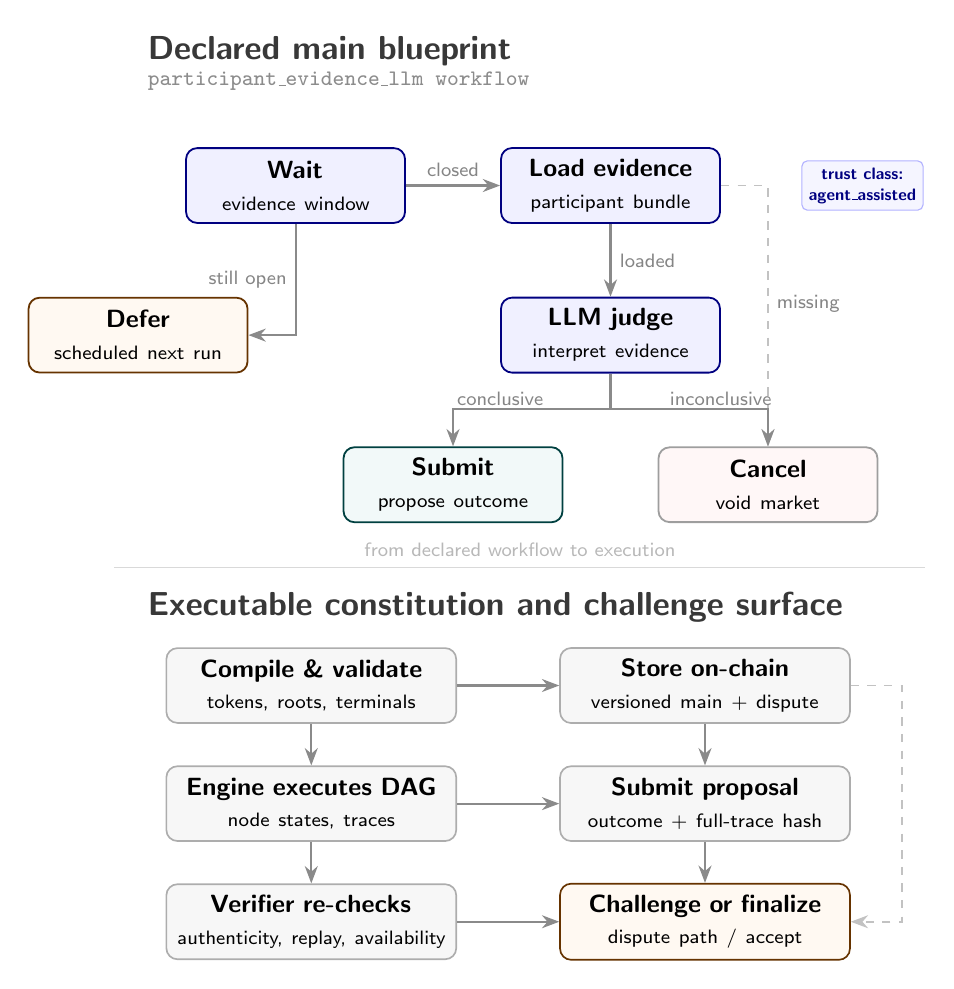
\begin{tikzpicture}[
  x=1cm, y=1cm,
  every node/.style={font=\sffamily},
  >={Stealth[length=2.2mm]},
  % ── DAG node styles ─────────────────────────────────────────────
  nbase/.style={
    text width=2.5cm, minimum height=0.95cm,
    align=center, inner sep=4pt,
    rounded corners=4pt, line width=0.65pt,
    font=\sffamily\fontsize{9pt}{10.5pt}\selectfont,
  },
  proc/.style={nbase, draw=blue!50!black, fill=blue!6},
  tsubmit/.style={nbase, draw=teal!50!black, fill=teal!5},
  tcancel/.style={nbase, draw=black!38, fill=red!3},
  tdefer/.style={nbase, draw=orange!40!black, fill=orange!5},
  % ── Stage styles (bottom half) ──────────────────────────────────
  sbase/.style={
    text width=3.4cm, minimum height=0.95cm,
    align=center, inner sep=4pt,
    rounded corners=4pt, line width=0.6pt,
    font=\sffamily\fontsize{9pt}{10.5pt}\selectfont,
  },
  stage/.style={sbase, draw=black!32, fill=black!3},
  sfinal/.style={sbase, draw=orange!40!black, fill=orange!5},
  % ── Labels and titles ──────────────────────────────────────────
  elabel/.style={
    font=\sffamily\fontsize{7pt}{8pt}\selectfont,
    text=black!48, inner sep=1pt,
  },
  ftitle/.style={
    font=\sffamily\bfseries\fontsize{12.5pt}{14pt}\selectfont,
    text=black!78,
  },
  fsubtitle/.style={
    font=\ttfamily\fontsize{7.6pt}{8.6pt}\selectfont,
    text=black!45,
  },
  sectitle/.style={
    font=\sffamily\bfseries\fontsize{11.5pt}{13pt}\selectfont,
    text=black!78,
  },
  badge/.style={
    draw=blue!30, fill=blue!4, rounded corners=2pt,
    font=\sffamily\fontsize{6.5pt}{7.5pt}\selectfont\bfseries,
    text=blue!50!black, inner sep=2.5pt, align=center,
  },
  % ── Arrows ─────────────────────────────────────────────────────
  flow/.style={->, line width=0.75pt, draw=black!46},
  faint/.style={->, line width=0.6pt, draw=black!24, dashed},
]

% ══════════════════════════════════════════════════════════════════
% TOP HALF: Worked blueprint DAG
% ══════════════════════════════════════════════════════════════════

\node[anchor=west, ftitle] at (0, 0.4) {Declared main blueprint};
\node[anchor=west, fsubtitle] at (0, 0.02) {\texttt{participant\_evidence\_llm} workflow};

% ── Row 0 (y = -1.3) ────────────────────────────────────────────
\node[proc] (wait) at (2, -1.3) {%
  \textbf{Wait}\\[1pt]{\scriptsize evidence window}};

\node[proc] (evidence) at (6, -1.3) {%
  \textbf{Load evidence}\\[1pt]{\scriptsize participant bundle}};

\node[badge] at (9.2, -1.3) {trust class:\\agent\_assisted};

% ── Row 1 (y = -3.2) ────────────────────────────────────────────
\node[tdefer] (defer) at (0, -3.2) {%
  \textbf{Defer}\\[1pt]{\scriptsize scheduled next run}};

\node[proc] (judge) at (6, -3.2) {%
  \textbf{LLM judge}\\[1pt]{\scriptsize interpret evidence}};

% ── Row 2 (y = -5.1) ────────────────────────────────────────────
\node[tsubmit] (submit) at (4, -5.1) {%
  \textbf{Submit}\\[1pt]{\scriptsize propose outcome}};

\node[tcancel] (cancel) at (8, -5.1) {%
  \textbf{Cancel}\\[1pt]{\scriptsize void market}};

% ── DAG edges (all orthogonal) ──────────────────────────────────

% Wait -> Evidence: horizontal
\draw[flow] (wait.east) -- node[elabel, above=2pt] {closed} (evidence.west);

% Wait -> Defer: down then left
\draw[flow] (wait.south) |- (defer.east);
\node[elabel, left=2pt] at (2, -2.5) {still open};

% Evidence -> Judge: straight down
\draw[flow] (evidence.south) -- node[elabel, right=2pt] {loaded} (judge.north);

% Evidence ~> Cancel: right then down (dashed)
\draw[faint] (evidence.east) -| (cancel.north);
\node[elabel, right=2pt] at (8, -2.8) {missing};

% Judge -> fork -> Submit / Cancel: symmetric Y-split
\path (judge.south) ++(0, -0.45) coordinate (fork);
\draw[flow, -] (judge.south) -- (fork);
\draw[flow] (fork) -| node[elabel, above, pos=0.35] {conclusive} (submit.north);
\draw[flow] (fork) -| node[elabel, above, pos=0.35] {inconclusive} (cancel.north);


% ══════════════════════════════════════════════════════════════════
% SEPARATOR
% ══════════════════════════════════════════════════════════════════

\draw[draw=black!15, line width=0.5pt] (-0.3, -6.15) -- (10, -6.15);
\node[font=\sffamily\fontsize{6.8pt}{7.8pt}\selectfont, text=black!28]
  at (4.85, -5.92) {from declared workflow to execution};


% ══════════════════════════════════════════════════════════════════
% BOTTOM HALF: Executable constitution and challenge surface
% ══════════════════════════════════════════════════════════════════

\node[anchor=west, sectitle] at (0, -6.65) {Executable constitution and challenge surface};

% ── Row 0 (y = -7.65) ───────────────────────────────────────────
\node[stage] (compile) at (2.2, -7.65) {%
  \textbf{Compile \& validate}\\[1pt]{\scriptsize tokens, roots, terminals}};

\node[stage] (store) at (7.2, -7.65) {%
  \textbf{Store on-chain}\\[1pt]{\scriptsize versioned main + dispute}};

% ── Row 1 (y = -9.15) ───────────────────────────────────────────
\node[stage] (run) at (2.2, -9.15) {%
  \textbf{Engine executes DAG}\\[1pt]{\scriptsize node states, traces}};

\node[stage] (proposal) at (7.2, -9.15) {%
  \textbf{Submit proposal}\\[1pt]{\scriptsize outcome + full-trace hash}};

% ── Row 2 (y = -10.65) ──────────────────────────────────────────
\node[stage] (verify) at (2.2, -10.65) {%
  \textbf{Verifier re-checks}\\[1pt]{\scriptsize authenticity, replay, availability}};

\node[sfinal] (dispute) at (7.2, -10.65) {%
  \textbf{Challenge or finalize}\\[1pt]{\scriptsize dispute path / accept}};

% ── Constitution flow (all orthogonal) ───────────────────────────

% Row 0: compile -> store (horizontal)
\draw[flow] (compile.east) -- (store.west);

% Col 0: compile -> run -> verify (vertical)
\draw[flow] (compile.south) -- (run.north);
\draw[flow] (run.south) -- (verify.north);

% Col 1: store -> proposal -> dispute (vertical)
\draw[flow] (store.south) -- (proposal.north);
\draw[flow] (proposal.south) -- (dispute.north);

% Cross: run -> proposal (horizontal)
\draw[flow] (run.east) -- (proposal.west);

% Cross: verify -> dispute (horizontal)
\draw[flow] (verify.east) -- (dispute.west);

% Dashed: store commitment enables challenge (orthogonal L-path)
\draw[faint] (store.east) -- ++(0.65, 0) |- (dispute.east);

\end{tikzpicture}
}
\caption{A declared participant-evidence workflow and its challenge surface. Waiting ends a run with defer; later execution follows the committed retry schedule. The evidence hash binds the full trace. The Boolean research profile separately tests authenticated report nodes, quorum routing, cancellation, and cross-run deferral.}
\label{fig:blueprint_constitution}
\end{figure}

The executable source-composition experiment uses $n=1$ or $n=3$ named report authorities and a strict-majority threshold $t$. Each report is Boolean or missing. All reports join before terminal selection. If at least $t$ authenticated reports agree, \texttt{submit\_result} emits that value. Otherwise the run defers when another authorized run remains, and cancels on the final run. A strict majority makes simultaneous opposite quorums impossible. Different source authorities and keys are required to count as distinct reports.

The profile rejects unknown fields and versions, duplicate node identities, invalid parent sets, inconsistent thresholds, cycles, and out-of-budget configurations. It permits at most 16 nodes and eight runs, with at most 262{,}144 canonical bytes per object. These are research-profile limits, not measurements of a deployed chain's capacity.

\subsection{Full-trace commitment and independent replay}

A run publishes a canonical trace $T$ binding the blueprint root, market and event identifiers, run number, previous run root, authenticated time anchors, every node's status, inputs, outputs and evidence references, the terminal action. An evidence object separately binds its source authority, request digest, event, market, run, node, observation time, and value. The proposed commitment is
\[
 h_T=\operatorname{SHA256}(\texttt{question.trace.v1}\,\|\,0\,\|\,C(T)),
\]
where $C$ is the profile's canonical encoding and $0$ is a zero-byte separator. Blueprint, request, and evidence hashes have distinct domain tags. This is a commitment to the entire reported run, not just its final context.

Canonical encoding is deliberately narrow: ASCII JSON strings and keys, sorted keys, no insignificant whitespace, ordered arrays, Boolean/null values and integers with magnitude at most $2^{53}-1$. Floats, duplicate keys, unknown fields, and noncanonical byte representations are rejected. Larger documents are referenced by digest; their byte encoding and authentication policy belong to the source specification.

The independent verifier retrieves the committed bytes, checks their hash and schema, reconstructs node order and inputs, authenticates evidence against the pinned keys and request scope, recomputes deterministic outputs and terminal routing, checks the complete set of records, and checks the retry chain and deadlines. It does not accept a node's declared output merely because the proposer hashed it. The prototype uses strict RSA-2048/SHA-256 verification for public test fixtures; all fixture private keys are intentionally published, and no production key or cryptographic implementation claim rests on them.

\begin{proposition}[Binding the executable constitution and reported run]
\label{prop:binding}
Assume an immutable commitment, a fixed interpreter and canonical encoding, and collision resistance of the tagged hash. Two different canonical specifications or traces cannot be substituted under the same respective commitment without a hash collision. Given a fixed authenticated input bundle, a deterministic verifier accepts at most the execution prescribed by the profile.
\end{proposition}
\begin{proof}
Distinct accepted canonical objects have distinct byte encodings. Equality of their tagged hashes is a collision. For replay, root inputs are fixed; induction along the stable topological order fixes each deterministic output, its status, and activated successors. Completeness fixes the record set, and the terminal rule fixes the action. The same induction applies to each authorized run after checking its predecessor and time anchor. External judgment is an input to this argument, not a conclusion of it.
\end{proof}

\subsection{Availability is a finalization condition}

A content identifier is not evidence that bytes can be retrieved. The executable profile therefore uses an explicit append-only publication layer with authoritative timestamps and publicly retrievable records. Source-slot admission checks the pinned signature before assigning a slot; arbitrary blobs cannot reserve another authority's slot. The first authenticated source publication and publication deadlines are binding. The trace and every referenced object must be available by their specified deadlines; missing or late material fails verification, even when the provided root is syntactically valid. An invalid proposal cannot finalize as a Boolean outcome. The declared market timeout routes unresolved execution to the cancellation policy.

This supplies an observable ``no trace, no finalization'' rule inside the model. In deployment the publication layer must be implemented by an available on-chain log, a data-availability service with an enforceable acceptance rule, or a named availability authority. That authority belongs in the trust profile. A CID alone cannot implement this check, and a prover's claim that publication occurred cannot replace the check.

\subsection{The challenge surface}

Blueprints make disputes specific. A verifier can challenge a commitment mismatch; a missing, duplicated, or reordered record; an unauthorized source or request; an invalid signature; an unavailable input; an unjustified branch; an incorrect deterministic output; an unauthorized retry; or a terminal outcome inconsistent with the recorded evidence. These are machine-checkable violations.

A correctly signed false statement and a faithfully reported bad judgment are different disputes. They can pass every structural check and still produce a wrong real-world result. The dispute blueprint specifies the independent evidence or authority used to judge them. The experiments preserve that separation: tampering is rejected, a fabricated consistent unsigned report fails authentication, and a quorum of genuinely signed false reports can pass replay. That last case is why source independence and dispute economics remain essential.

\section{Trust Classes}
\label{sec:trustclasses}

A participant should know before trading whether the declared workflow relies on source data, machine judgment, human judgment, or a fallback that changes that answer. The blueprint exposes those dependencies automatically.

\subsection{Classification function}

For the union of the main and dispute programs, let $T(G)$ be its node types. Define
\[
\kappa(G)=\begin{cases}
\texttt{human\_judged},&\texttt{human\_judge}\in T(G),\\
\texttt{agent\_assisted},&\texttt{llm\_judge}\in T(G)\text{ otherwise},\\
\texttt{source\_based},&\text{otherwise}.
\end{cases}
\]
The label is computed syntactically over all declared nodes, including fallback paths. Adding a human-judgment node cannot hide it beneath a source-only label. This monotonicity is immediate from the definition; the ordering is label precedence, not a ranking of safety. A rigorous human panel can outperform an unauthenticated API. A source-only workflow with a human dispute fallback must disclose both.

The full trust profile is the operational object:
\[
\chi(G)=(\kappa,\;\mathcal A,\;\mathcal U,\;r,\;d,\;a,\;f,\;v),
\]
where $\mathcal A$ names source and judgment authorities and their authentication rules; $\mathcal U$ records known common dependencies; $r$ states the replay/authentication boundary; $d$ specifies availability and deadlines; $a$ and $f$ specify adjudication and fallback; and $v$ pins semantics and change authority. A parser can derive declared dependencies. It cannot prove that two providers have no undisclosed common owner or upstream source. Declared independence is tested as a threat-model input, not certified from different endpoint strings.

\subsection{What the classes mean}

\textbf{Source-based.} Extraction and decision logic are deterministic relative to declared source objects. The profile states whether those objects are authenticated, merely archived, or reported by the executor.

\textbf{Agent-assisted.} A model supplies a judgment. Its provider, model identifier, prompt, parameters, input-evidence rule, output schema, and serving attestation are part of the specification. The verifier can check the declared interface and subsequent routing. A nondeterministic verdict is not disproved merely because another model call disagrees.

\textbf{Human-judged.} A named person or panel supplies a judgment under a declared rubric and evidence policy. Identity, quorum, conflicts policy, and dispute route are visible assumptions. Human judgment need not be reproducible to have a rigorous interface and an accountable record.

The class is the headline. The executable constitution and the trace make the headline inspectable.

\subsection{Composition, bias, and credibility}
\label{sec:llmbias}

A blueprint can combine sources and judges, require corroboration, and route disagreement to cancellation or escalation. This raises attack cost when an attacker must control more independent authorities to reach a wrong terminal. Section~\ref{sec:composition} proves that statement as a minimum-cost authority cut and tests it by corrupting actual source objects before executing the program.

The same construction exposes its own failure cases. Three feeds backed by one compromised upstream do not provide three independent barriers. Two models prompted from the same poisoned evidence can agree on the same mistake. A serving signature proves which provider issued a response, not that the response is true. The protocol therefore commits both the aggregation rule and the authority structure; the empirical tests include shared-upstream corruption and withheld evidence. The strength of composition is a measurable property of that structure, not a benefit assigned to a label in the simulator.

\section{Dispute Economics}
\label{sec:dispute}

A blueprint makes the promise explicit. Dispute economics make keeping that promise rational. A protocol needs a willing proposer, an actual checker, liquid challenge capital, and an adjudicator capable of correcting the error. None of those services appears merely because a contract exposes a function.

\subsection{A funded resolution game}

Consider a binary market with collateral $L$ and true outcome $0$. Participant $i$ has funded payout claims $\pi_i(0),\pi_i(1)\geq0$ satisfying
\[
\sum_i\pi_i(0)=\sum_i\pi_i(1)=L.
\]
The gain from false resolution is the \emph{signed} difference
\[
D_i=\pi_i(1)-\pi_i(0),\qquad -L\leq D_i\leq L.
\]
A holder of only the true winning claim has $D_i<0$. Treating its absolute position as an incentive to lie reverses the economics. Bond capital $K_i$ is liquid wealth separate from these locked claims.

A proposer posts $B_P$ and incurs work and capital cost $c_P$. A prepaid reserve supplies fee $F$ if the proposal survives adjudication. A challenger posts $B_C$ and incurs filing and capital cost $c_C$. When a challenge succeeds, the proposer loses $B_P$, the challenger receives $\eta B_P$, and the protocol receives $(1-\eta)B_P$, where $0\leq\eta\leq1$. The unused fee remains in the reserve. When a challenge fails, its bond goes to the protocol; the proposer receives its own bond back and $F$. Bonds returned to their owners are not rewards.

The actors are risk-neutral. Adjudication returns the true outcome with probability $a$. Work costs are resource costs, capital costs are opportunity costs, and bonds and fees are transfers. Every realized branch balances the participant accounts, protocol account, and prepaid reserve separately from resources consumed. No bounty is created by minting an unbacked percentage of market value.

\subsection{Challenge decisions and dishonest challenges}

After inspecting proposal $x\in\{0,1\}$ and learning the truth, challenger $j$ compares filing with accepting the proposal at its submission opportunity. Write $v_1=a$ and $v_0=1-a$ for the probability that adjudication overturns the proposed answer. Its incremental filing value is
\begin{equation}
C_j(x)=v_x\bigl[\pi_j(1-x)-\pi_j(x)+\eta B_P\bigr]
       -(1-v_x)B_C-c_C.
\label{eq:challenge}
\end{equation}
Inspection cost is already sunk at this point. Filing requires both $C_j(x)>0$ and enough liquid capital to cover the bond and incurred work. Thus a participant may challenge a false result to recover its payout, challenge for the bond reward without a position, or even challenge a true result when adjudicator error and its false-outcome exposure make doing so profitable. The model allows all three. It does not grant honest proposals immunity from checking or griefing.

Let $q_x$ be the probability that proposal $x$ receives such a challenge under the declared inspection policy. In the operational experiments this is computed from the same capital and payoff gates used for realized filing. For independent eligible checkers with inspection probabilities $p_j$ and probability $d_j$ of learning proposal validity,
\[
q_x=1-\prod_{j\ne P:\,C_j(x)>0,\ K_j\text{ sufficient}}(1-p_jd_j).
\]
The model below separately asks whether neutral inspectors will voluntarily supply those inspections.

\subsection{Proposer choice and the deterrence frontier}

Relative to receiving the truthful market payout without providing proposal work, a proposer's expected incremental payoffs are
\begin{align}
U_0&=F-c_P+q_0(1-a)(D-B_P-F),\label{eq:truthful_utility}\\
U_1&=D+F-c_P-q_1a(D+B_P+F).\label{eq:false_utility}
\end{align}
An eligible proposer chooses the largest of truthful submission, false submission, and the zero incremental outside option. The operational outside option is waiting or relying on another resolver; if everyone abstains, the episode is deferred, not recorded as correct. A willingness calculation is therefore distinct from a liveness outcome.

The clean deterrence result concerns a neutral-monitor regime: honest proposals are not falsely challenged ($q_0=0$), an actual challenge reaches the true answer with probability $a$, and work costs are the same for true and false submissions. Define effective correction probability $r=aq_1$.

\begin{theorem}[False-proposal deterrence]
\label{thm:deterrence}
In this regime the advantage of lying over truthful submission is
\begin{equation}
\Delta=(1-r)D-r(B_P+F).
\label{eq:deterrence}
\end{equation}
For $D>0$ and $r>0$, truthful submission weakly dominates lying exactly when
\begin{equation}
B_P+F\ \geq\ \frac{1-r}{r}D,
\qquad\text{equivalently}\qquad
r\ \geq\ \frac{D}{D+B_P+F}.
\label{eq:frontier}
\end{equation}
If $r=0$ and $D>0$, no finite bond deters the lie. For $D\leq0$, lying supplies no positive outcome-exposure advantage in this regime.
\end{theorem}
\begin{proof}
Subtract~\eqref{eq:truthful_utility} with $q_0=0$ from~\eqref{eq:false_utility}. Successful correction removes the false payout gain, slashes the bond, and forfeits the accepted-proposal fee. Rearrangement gives~\eqref{eq:frontier}. With $r=0$, the bond is never at risk and $\Delta=D$.
\end{proof}

This equation is the design rule. A large bond and a sophisticated arbitrator cannot compensate for zero checking. Conversely, effective checking makes a moderate bond meaningful. When honest proposals can be falsely challenged, the simulator uses both full utilities above; the restricted theorem is not silently applied to that larger game.

\begin{corollary}[Why flat bonds fail at scale]
\label{cor:scaling}
Suppose a family of markets permits $D(L)\geq\kappa L$ for some $\kappa>0$, while $r(L)\leq\bar r<1$. If $B_P(L)+F(L)=o(L)$, truthful submission eventually ceases to dominate false submission. If the fee remains sublinear, the bond must scale with exposure to maintain deterrence.
\end{corollary}
\begin{proof}
Equation~\eqref{eq:deterrence} gives
$\Delta\geq(1-\bar r)\kappa L-\bar r(B_P+F)$, which is positive for sufficiently large $L$. A fixed bond or a binding fixed cap is a special case.
\end{proof}

Pool collateral is a conservative bound in this funded single-market game, not a substitute for measuring exposure. Diffuse, enforceably bounded positions can justify a smaller $D$; concentrated or connected external positions can require a larger one. Splitting ownership across addresses does not enforce an economic exposure bound. A large success fee can also supply deterrence through its forfeiture, but it must be funded: the theorem concerns $B_P+F$, not the bond in isolation.

\subsection{Coverage and adjudication are complementary}

Conditional on a false proposal, the probability of a wrong final result is
\begin{equation}
1-aq=(1-q)+q(1-a).
\label{eq:failure_decomposition}
\end{equation}
The first term is failure to challenge; the second is adjudication failure after a challenge. Coverage failure dominates precisely when
\[
q<\frac{1}{2-a}.
\]
At $a=0.95$, that threshold is about $0.9524$. Thin-market coverage is therefore a severe bottleneck across a wide regime. The marginal reduction in wrong results from raising $q$ is $a$; from raising $a$ it is $q$. When $q\ll a$, an equal absolute improvement in coverage has the larger effect. At high coverage, adjudication becomes the binding limit: $q\leq1$ implies $r\leq a$. The paper's operational conclusion is to fund missing checking capacity, while preserving an explicit accuracy target for the dispute path.

\subsection{The lazy verifier problem as an inspection game}
\label{sec:monitoring}

Consider $n$ capital-eligible, neutral inspectors, each available with probability $u$. An available inspector chooses verify, shirk, or idle. Verification costs $c>0$ on \emph{every} proposal, including a truthful one. A verification retainer pays $w$ for a valid completion claim. A posted performance bond $S$ incurs opportunity cost $k_S$. An independent audit detects skipped work with probability $\delta$, withholds $w$, and slashes $S$; the baseline audit makes no false accusations. The audit condition means skipped work is actually testable. It is an assumption about the work contract, not something a self-authored trace proves.

A detected false proposal yields net challenge surplus
\[
R=a\eta B_P-(1-a)B_C-c_C.
\]
The neutral subgame also requires false challenges to be unprofitable: $T=(1-a)\eta B_P-aB_C-c_C\leq0$, with no challenge on a tie. A viable corrective challenge requires $R>0$ and capital sufficient for $B_C+S$ under the model's work-funding convention. If $m$ is the probability an available inspector verifies, coverage and its probability of winning the first-challenger reward conditional on verifying are
\begin{equation}
q(m)=1-(1-um)^n,\qquad
A(m)=\frac{1-(1-um)^n}{num},
\label{eq:inspection}
\end{equation}
with $A(0)=1$. Ties are awarded uniformly among actual inspectors. If fraud occurs with probability $f$, the available inspector's utilities are
\[
V=w-c-k_S+fR A(m),\qquad
H=(1-\delta)w-\delta S-k_S,\qquad I=0.
\]
The equilibrium balances verification against $\max(H,0)$, so the effective cost of inspection is
\[
k=c-w+k_S+\max\{0,(1-\delta)w-\delta S-k_S\}.
\]
Capital scarcity reduces $n$; availability limits maximum coverage to $q_{\max}=1-(1-u)^n$. Neither a high posted reward nor many registered identities guarantees a high $n$ or $u$. Equations~\eqref{eq:inspection} assume no common outage. With common outage probability $z$, coverage is $(1-z)[1-(1-um)^n]$; $A(m)$ is unchanged conditional on the inspector being available. The proposer does not observe the outage before acting.

\begin{proposition}[Discrepancy rewards require discrepancies]
\label{prop:rare_fraud}
For neutral, costly inspectors with $w=S=k_S=0$, an all-truthful state cannot sustain positive voluntary inspection solely through fraud bounties. With no common outage ($z=0$) and truthful participation $F\geq c_P$, an interior mixed equilibrium, when it exists, satisfies
\[
q^*=\frac{D}{a(D+B_P+F)},\qquad
m^*=\frac{1-(1-q^*)^{1/n}}{u},\qquad
f^*=\frac{c}{R A(m^*)}.
\]
These expressions apply only when $0<m^*,f^*<1$ and the challenge and capital gates hold. The released solver selects a symmetric equilibrium with explicit tie rules and checks every pure-action deviation; it does not claim equilibrium uniqueness.
\end{proposition}
\begin{proof}
At $f=0$, verification yields $-c<0$, whereas idling yields zero; therefore voluntary inspection vanishes. With $D>0$ and no checking, lying is profitable relative to truthful submission. At an interior equilibrium the proposer is indifferent by~\eqref{eq:frontier}, giving $q^*$ and then $m^*$. Inspector indifference gives $f^*RA(m^*)=c$.
\end{proof}

This is the structural reason a large fraud bounty cannot, by itself, guarantee continuous inspection in a quiet market. A rare-fraud equilibrium can have low error, but it does not purchase an unconditional checking service.

\begin{proposition}[A funded truthful-inspection regime]
\label{prop:paid_inspection}
Suppose $D>0$, $R>0$, $T\leq0$, the proposer has free bond capital at least $B_P$, and $n$ inspectors have capital at least $B_C+S$. Assume the required external reserve is prepaid, service work costs are accounted for separately from free bond capital, and an auditable work contract satisfies
\begin{equation}
w>c+k_S,\qquad \delta(w+S)>c.
\label{eq:work_ic}
\end{equation}
Use $q_{\max}=(1-z)[1-(1-u)^n]$, with $z=0$ in the independent-availability case. If $a q_{\max}>D/(D+B_P+F)$ and $F>c_P$, then available inspectors strictly prefer verification to shirking and idling even when $f=0$, and the proposer strictly prefers truthful submission to false submission and abstention in the neutral-monitor subgame.
\end{proposition}
\begin{proof}
At zero fraud, $V>0$ by the first inequality and $V-H=\delta(w+S)-c>0$ by the second. Every available inspector verifies, giving $q_{\max}$. The strict frontier inequality deters lying, and $F>c_P$ makes truthful work profitable. A prepaid reserve of at least $F+n(w+c_A)$ covers the worst-case proposal fee, retainer payments, and per-inspector audit cost $c_A$; slashed bonds are transfers rather than an assumed source of recurring work funding.
\end{proof}

Paying without enforcing work fails this construction. With $\delta=0$ and no effective performance bond, shirking collects the same retainer while saving $c$. The simulator includes that control. Sybil creation likewise cannot multiply paid slots: the work contract admits a funded set of distinct audit assignments, with a fixed total reserve. Establishing credible assignments and audits for subjective judgments is a product requirement; the theorem makes that requirement explicit and measurable.

\begin{corollary}[Paid work without additional collateral exclusion]
\label{cor:zero_stake}
In the neutral-inspector game with $T\leq0$, retain the bounty-only population and capital budgets, set $S=0$, $\delta=1$, and $w>c$, and prepay the required reserve. All available eligible inspectors strictly verify. With profitable truthful participation and truthful choice on a payoff tie, the selected equilibrium's wrong-finalization rate is no greater than under bounty-only inspection.
\end{corollary}
\begin{proof}
No work stake changes eligibility. Verifying yields at least $w-c>0$, while shirking and idling yield zero. Thus the new challenge coverage is $q_{\max}$, defined as zero when $R\leq0$. If it reaches the deterrence frontier, the proposer selects truth and the wrong rate is zero. If it falls short, fraud is profitable even at maximal coverage, so both policies select fraud; $1-aq_{\max}\leq1-aq_{\rm bounty}$. Nonpositive signed exposure selects truth. Reserve sufficiency prevents a new no-launch outcome.
\end{proof}

This is a constructive alternative when scarce challenge capital makes an extra performance stake counterproductive. It buys enforceable auditing and routine work from an external budget. The gain depends on the audit technology; full auditing is not assumed to be free or universally available.

\subsection{Proposer compensation and liveness}

A neutral truthful proposer in the no-griefing regime earns $F-c_P$, where a useful cost model is
\[
c_P=c_{\rm work}+\iota B_P\frac{T_P}{8760}.
\]
Here $\iota$ is an annual capital rate and $T_P$ a committed lock duration in hours. If $F<c_P$, returning the bond leaves the proposer worse off. If no eligible proposer accepts that loss, no proposal arrives. A correct cancellation requires work too and should earn the declared service fee when that is the blueprint's valid terminal action. Compensation and collateral solve different problems: the fee buys honest service; the bond makes successful cheating costly.

Larger bonds can price casual proposers and challengers out of the market. The experiments therefore report liquid-capital eligibility, willingness, submission, and deferral separately. Reducing a bond to restore participation can move the market below its deterrence frontier. The alternative is to fund service and challenge capacity commensurate with the exposure.

\subsection{A challenge window must buy a coverage target}

For independent challenge-capable arrivals at aggregate rate $\Lambda$ after complete evidence is available,
\[
q(W)=1-e^{-\Lambda W}.
\]
Combining this with~\eqref{eq:frontier} gives, for $0<q_{\rm req}<1$,
\begin{equation}
q_{\rm req}=\frac{D}{a(D+B_P+F)},\qquad
W\geq\frac{-\log(1-q_{\rm req})}{\Lambda}.
\label{eq:window}
\end{equation}
If $q_{\rm req}>1$, no window suffices; if $q_{\rm req}=1$, Poisson arrival requires an infinite window. If evidence arrives late, the effective interval is shorter. Adjudication delay and capital cost must also be funded. Thus 24 hours has no universal economic status: the required time follows from exposure, bonds, accuracy, trace availability, and measured arrival capacity.

For example, with $D=L$, $F=0$, and $a=0.9$, a bond of $0.10L$ requires $q\approx1.0101$ and cannot deter the worst-case holder. A bond of $0.15L$ requires $q\approx0.9662$. These are exact frontier calculations. The protocol should publish the target and the capacity needed to meet it, rather than advertise a percentage without its checking requirement.

\subsection{What escalation adds}

A sequential dispute path must be analyzed as a sequence of funded opportunities to correct a still-wrong proposal. Suppose stage $j$ corrects it with conditional probability $r_j$ given survival to that stage. Correct resolution is absorbing. Write $S_0=1$ and $S_j=\prod_{i=1}^{j}(1-r_i)$. If earlier bonds are returned, only $B_j$ is lost at the first correction, the accepted-proposal fee $F$ is forfeited on correction, and all stages are financially feasible, the fraud advantage is
\[
\Delta_{\rm seq}=S_JD-\sum_{j=1}^{J}S_{j-1}r_j(B_j+F)-\Delta c,
\]
where $\Delta c$ is the fraud strategy's additional expected work and capital cost relative to truthful submission. This identity follows by partitioning on the first correction stage; it needs no independence assumption. If $\Delta c\geq0$, dropping it gives a conservative deterrence bound. The correction probabilities must incorporate actual attendance, capital, and accuracy at each stage. Calling a single low initial bond an ``escalation game'' does not supply those probabilities. The one-shot numerical comparisons in this paper are not a ranking of unimplemented sequential dispute systems.

\subsection{Composition raises the cost of corrupting inputs}
\label{sec:composition}

Let a deterministic blueprint accept a Boolean answer exactly when at least $t$ of $n$ distinct source authorities report it, with $t>n/2$. Assume otherwise correct and available sources, fixed request binding, no executor forgery, and independent source control with costs $c_1,\ldots,c_n>0$. Let $c_{(1)}\leq\cdots\leq c_{(n)}$ be the sorted costs.

\begin{proposition}[Threshold corruption cost]
\label{prop:source_cost}
The minimum cost of producing an accepted wrong answer is
\[
C_{\rm wrong}=\sum_{j=1}^{t}c_{(j)}.
\]
With a strict majority, withholding alone cannot create a wrong quorum. It can still destroy liveness by removing enough correct reports.
\end{proposition}
\begin{proof}
A wrong accepted answer contains at least $t$ distinct authenticated wrong reports, so the attacker must pay for at least $t$ authorities. The cheapest such set costs the stated sum. Corrupting exactly those authorities and reporting the wrong value attains the bound. Missing reports do not count as wrong reports, so withholding cannot satisfy the wrong-value threshold.
\end{proof}

For shared dependencies, assign costs to independent \emph{control domains} instead of endpoint names. If compromising domain set $A$ controls source set $S(A)$, the bound becomes
\[
C_{\rm wrong}=\min_{A:\,|S(A)|\geq t}\sum_{z\in A}c_z.
\]
This is a weighted authority-cover problem. A common upstream that controls two of three reports can collapse the threshold cost to one domain's price. Our experiments enumerate feasible corruptions and withholding choices, execute the resulting reports, and compare measured terminal outcomes with this bound. Deterrence, blocked execution, cancellation, and wrong finalization remain distinct outcomes.

\section{Simulation Program}
\label{sec:simulation}

The experimental program separates three questions: how funded participants respond to a specified checking service, whether inspectors will provide that service, and whether the blueprint actually rejects or accepts manipulated evidence. Each has its own executable model and evidence artifacts. Source resilience is never inserted as an unexplained probability multiplier in the economic game.

\subsection{Funded participants and operational checking}

The main experiment runs 171 configurations, 20 seeds per configuration, and 250 episodes per seed: 855{,}000 episodes. Seeds 64000--64019 and the full parameter grid are recorded before the final run. All treatments share latent participant, arrival, detection, and adjudication draws. Development smoke tests preceded that freeze; this is a locally frozen design, not an externally preregistered study.

Each episode assigns exclusive binary claims to two nonempty groups and normalizes each outcome's total payout to $L$. Position weights are uniform, rank weights $i^{-0.8}$, or a concentrated vector with one pre-normalization weight $0.6$ and the others sharing $0.4$. Truth-side membership is randomized. Free capital is independent of those funded positions. The capital stress profiles use declared synthetic mixtures of log-uniform bands: retail, mixed, specialized, and an unconstrained control. They model access constraints rather than estimate the wealth of actual users.

The default market has ten participants, $L=5000$, $B_P=0.15L$, $B_C=B_P$, $\eta=0.5$, adjudicator accuracy $0.95$, a 24-hour window, and a further 24-hour capital-lock reserve. Work costs are 2 for proposing, 0.5 per inspection, and 0.25 per challenge, with a 20\% annual capital rate. Except in explicit compensation and griefing experiments, the fee rule is
\[
F=\max\{5,\ c_{\rm proposal\ work}+c_{\rm proposal\ capital}+1\}.
\]
Bond and window interventions therefore retain funded truthful service; they do not conceal a loss of liveness behind a lower error rate.

Provisioned inspection readiness follows exponential arrival. High-attention rates are uniform on $[0.05,0.15]$ per hour. Low attention is a mixture: 15\% draw from $[0.01,0.03]$, and the remainder from $[0.0005,0.003]$. A third policy scales the rate with the participant's payout exposure. Scheduled inspections occur on honest and false proposals, all completed work within the window is charged, and the first ready capital-eligible participant with positive filing value challenges. These are operational service policies. The separate equilibrium experiment supplies the endogenous checking analysis.

All eligible candidates evaluate the same true/false/abstain utilities used by execution. The baseline selects the first willing candidate in an independent random priority order; an adversarial selection treatment gives priority to willing fraud. The eleven families cover bond scaling, caps, windows, accuracy, reward allocation, position concentration, compensation, honest-proposal griefing, thin attention, challenge-capital access, and proposer selection.

Position concentration changes both the largest individual incentive and the population of willing proposers; it need not monotonically raise average error. The recorded endpoints distinguish no submission, correct resolution, wrong resolution, attempted fraud, false challenge, wrongful slashing, and positive-gain candidates deterred into truthful submission. Wrong outcomes are reported both per episode and conditional on submission. Resource costs, capital costs, transfers, and payout redistribution are separate quantities.

\subsection{Endogenous inspection and funded work}

The monitoring model solves the verify/shirk/idle game exactly in 15 designed configurations (the principal policies and stress controls) and 64 fresh synthetic parameter regimes. Each fresh regime has bounty-only, paid unaudited, and paid audited arms. The 64 regimes are generated by seed 908731 across exposure, bond ratios, capital supply, availability, accuracy, checking cost, and common outages. All 192 fresh arm results are retained, including harmful interventions.

Three Monte Carlo seeds (730001, 730003, 730009), each with 20{,}000 episodes per designed configuration, independently check the exact expectations: 900{,}000 episodes. Every episode checks money conservation and the reserve ceiling. The first 100 episodes per seed/configuration are retained as readable traces; the entire stream is reproducible from the recorded seeds. All exact equilibria are checked against pure-action best responses, including shirking and abstention.

Availability is independent across inspectors conditional on common uptime. The proposer acts before observing outages. Work-audit detection is an explicit external technology; the model does not infer genuine effort from a self-reported receipt. The full funded participant game allows profitable false challenges; the neutral-inspector subgame rejects parameterizations in which that omitted action would be profitable.

\subsection{Executed evidence corruption}

The blueprint suite executes and independently verifies all 30 one-source and three-source Boolean-or-missing input vectors. Forty finite-state experiments expand to 1{,}670 weighted rows, with exact rational probabilities. They cover independent source error, a common upstream error at matched marginal accuracy, independent and common outages, forced corruption, withholding, and budget-constrained attacker choice before or after observing latent errors and availability.

The attacker changes actual source objects or withholds them. The interpreter then selects submit, defer, or cancel. The independent checker validates that emitted trace. Additional attack vectors alter identities, signatures, scope, node records, outcomes, roots, publication timing, and retry history. A fabricated internally consistent trace and an authentically signed common-source error are explicit negative controls. These experiments test executable structure and specified source processes; they do not measure real-world hacking prices or live model accuracy.

\subsection{Uncertainty and reproducibility}

Economic rates include Wilson intervals. Treatment differences use paired seed means with a 95\% Student-$t$ interval over 20 seed clusters. The complete grid is reported; these are pointwise simulation intervals, not multiplicity-adjusted discoveries or uncertainty bounds on human behavior. Source-state results are exact conditional expectations and need no Monte Carlo interval. Monitoring equilibria are exact numerical solutions, checked separately by simulation.

Every economic episode records exact conditional wrong-outcome probability alongside its realized outcome, allowing an independent expectation-versus-sampling check. The largest absolute standardized discrepancy across 171 configurations was 1.88; the largest cash-balance residual was below $1.5\times10^{-12}$ monetary units. Monitoring best-response regret was below $2.9\times10^{-14}$ and money imbalance below $1.5\times10^{-15}$. Independent branch-enumeration tests check both honest and false proposals. Frozen configurations, source hashes, raw economic episodes, exact weighted source states, test vectors, and reproduction commands accompany the manuscript. Historical outputs remain archived and are not inputs to these results.

\section{Results}
\label{sec:results}

\subsection{Flat bonds fail as exposure grows}

Table~\ref{tab:bond_results} shows the low-attention scaling experiment. At $L=5000$, replacing a flat bond of 10 with $0.15L$ reduces wrong outcomes from 63.06\% to 28.14\%, a paired change of $-34.92$ percentage points (95\% interval $[-36.05,-33.79]$). At $L=50{,}000$ the corresponding change is $-34.84$ points ($[-36.00,-33.68]$). Submission remains 100\% in these unconstrained-capital comparisons.

\begin{table}[t]
\centering
\caption{Wrong outcomes per episode under low attention. Each cell uses 5{,}000 paired episodes. All episodes submit; deferral is zero. The fee follows the declared service-cost rule.}
\label{tab:bond_results}
\small
\begin{tabular}{rrrrr}
\toprule
Collateral $L$ & Flat 10 & $0.10L$ & $0.15L$ & $0.50L$ \\
\midrule
50 & 21.08\% & 21.08\% & 21.08\% & 0.72\% \\
500 & 30.54\% & 29.38\% & 27.74\% & 2.66\% \\
5{,}000 & 63.06\% & 29.60\% & 28.14\% & 2.98\% \\
50{,}000 & 63.06\% & 29.62\% & 28.22\% & 3.00\% \\
\bottomrule
\end{tabular}
\end{table}

Proportional bonds improve scale behavior but do not manufacture coverage. Even a 50\% bond leaves wrong outcomes in the low-attention policy. Under high attention, the proportional-bond treatments deter false proposals in this grid. Flat bonds create another problem: at $L\geq5000$, honest proposals are challenged opportunistically and adjudication errors produce a 4.94\% wrong-outcome rate. The model now exposes both the fraud-deterrence and honest-defense roles of adequate collateral.

\begin{figure}[t]
\centering
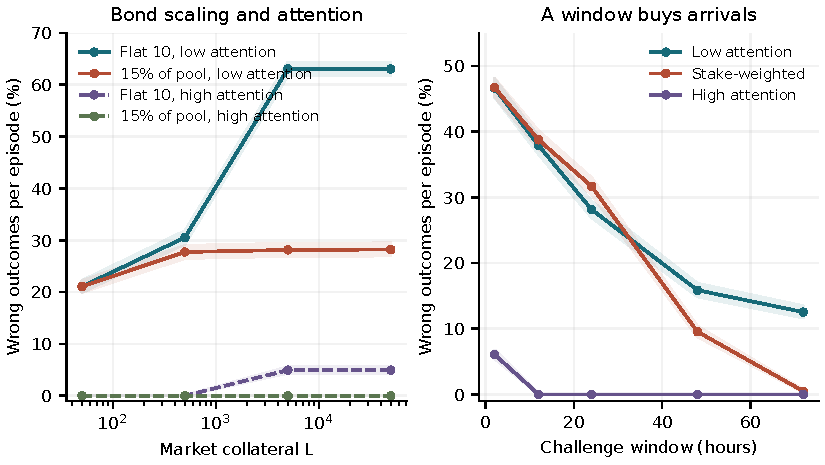
\includegraphics[width=\linewidth]{funded_game.pdf}
\caption{Funded-game comparative statics. Left: flat and proportional bonds across scale and attention. Right: longer windows purchase more inspection arrivals, with different returns under each policy. Shading shows 95\% Wilson intervals; these quantify conditional Monte Carlo uncertainty.}
\label{fig:funded_results}
\end{figure}

A bond cap can restore capital access while reducing integrity. At $L=50{,}000$ with mixed capital, an uncapped 15\% bond yields 98.08\% submission and 42.42\% wrong outcomes per episode. A cap of 250 restores submission to 100\% but raises wrong outcomes to 63.06\%. Other caps change both who can challenge and who will propose, so aggregate error is not monotone in the cap. The theorem's exposure frontier remains the appropriate safety criterion.

\subsection{Coverage is the thin-market bottleneck}

With low attention at $L=5000$, raising accuracy from 0.95 to 1 reduces wrong outcomes only from 28.14\% to 26.62\%, a paired change of $-1.52$ points ($[-1.91,-1.13]$). Perfect adjudication cannot repair proposals nobody challenges. Extending the window from 24 to 48 hours instead reduces wrong outcomes to 15.86\%, a change of $-12.28$ points ($[-13.29,-11.27]$); 72 hours reaches 12.52\%. High-attention markets in the same sweep are already deterred at 12 hours. There is no universal 24-hour plateau.

The bound in Figure~\ref{fig:frontier_composition} makes the mechanism explicit. Coverage and adjudication multiply; a bond percentage without a coverage target is incomplete. In the operational reward-allocation sweep, changing $\eta$ from zero to one produces no outcome change at the sampled participant counts: exposed participants already find correction worthwhile, while readiness is provisioned independently of the reward. That null result is useful. The endogenous inspection game is where a reward can change whether checking happens.

\subsection{Pay for checking, and make checking preferable to shirking}

For the designed monitoring example, $L=10{,}000$, $D=4000$, $B_P=B_C=1500$, $a=0.95$, and $F=20$. Three inspectors each have availability 0.6, inspection cost 2, and sufficient capital. The paid arms use $w=3$ and $S=2$; the audited arm has $\delta=0.5$. Table~\ref{tab:monitoring} reports exact equilibria.

\begin{table}[t]
\centering
\caption{Exact inspection equilibria. Coverage is conditional on a false proposal; wrong rate is per offered episode. Spend is the expected external fee, work-payment, and audit budget used. No-submission controls are reported separately in the text.}
\label{tab:monitoring}
\small
\begin{tabularx}{\linewidth}{@{}Yrrrr@{}}
\toprule
Policy & Fraud & Coverage & Wrong & Spend \\
\midrule
Bounty only & 0.4719\% & 76.28\% & 0.1299\% & 19.93 \\
Paid, unaudited & 0.4719\% & 76.28\% & 0.1299\% & 25.33 \\
Paid, audited & 0\% & 93.60\% & 0\% & 25.58 \\
Audited, 30\% common outage & 100\% & 65.52\% & 37.756\% & 11.46 \\
Audited, no challenge capital & 100\% & 0\% & 100\% & 20.00 \\
\bottomrule
\end{tabularx}
\end{table}

The unaudited retainer raises expenditure without changing fraud or coverage: 36.51\% of available inspectors shirk. With the audit, verifying strictly beats shirking and idling. Coverage exceeds the deterrence frontier, and truthful submission becomes the equilibrium. The worst-case reserve is 29.60, so the construction is fully funded. Removing the proposer fee produces no profitable submission; cutting the reserve below its required value prevents launch. Neither is scored as a correct resolution.

The fresh 64-regime test identifies the capital tradeoff. Holding the retainer, work stake, and free capital fixed, adding the audit lowers mean wrong outcomes by 6.94 points: 12 regimes improve and 52 tie, with none worsening. But comparing the entire paid-audited package against bounty-only raises mean wrong outcomes by 2.50 points across all 64 regimes. The work stake excludes some inspectors in 40 regimes; all 16 worsening cases lose eligible inspectors. Buying accountable work while taking away challenge capacity can defeat the intervention. The constructive requirement is to satisfy the work, capital, reserve, and coverage inequalities together.

A subsequent mechanism experiment applies Corollary~\ref{cor:zero_stake} to all 64 original regimes: retain their free capital and other parameters, set $S=0$, pay $w=1.25c$, and audit every claimed completion. This follow-up was designed after observing the capital tradeoff and is reported separately from the original three-arm study. All 64 regimes retain their baseline eligible-inspector count and meet the reserve requirement. Mean wrong finalization falls from 49.10\% under bounty-only to 40.72\%: 18 regimes improve, 46 tie, none worsen. Mean external expenditure rises from 5.63 to 14.48. The construction purchases greater integrity with funded, enforceable work instead of extra challenge-capital exclusion; it does not turn the assumed audit technology into a field result.

\subsection{Compensation converts willingness into service}

At $L=5000$ with mixed capital and proposal work cost 10, moving $F$ from 0 to 15 raises submission from 96.10\% to 100\% and reduces wrong outcomes from 66.90\% to 29.18\%. The paired wrong-outcome change is $-37.72$ points ($[-38.67,-36.77]$). With no fee, the willing service providers in this regime are motivated by false-outcome gains. Funding honest service changes the proposer population.

At $L=50{,}000$ with mixed capital, $F=50$ raises submission from 83.64\% to 98.08\% and reduces wrong outcomes from 72.82\% to 41.74\%. Retail capital remains scarce: with the same fee, only 29.74\% of episodes submit, and 14.60\% of all episodes resolve wrongly. The latter number is not a safety improvement; conditional on submission, wrong resolution is about 49.09\%. A funded service fee does not create collateral capacity.

\subsection{Challenge access and proposer selection matter}

Reducing the challenge bond admits more challengers but also cheaper false challenges. In the honest-proposer, concentrated-position test with $a=0.9$, setting $B_C=0.001B_P$ produces 4.36\% wrong outcomes despite every submitted proposal being true; the equal-bond control produces none. The paired difference is $4.36$ points ($[3.83,4.89]$). Challenge access must be designed against both suppression of valid disputes and griefing of valid results.

Proposer selection is equally material. In the low-attention uniform-position baseline, random first-willing selection yields 28.14\% wrong outcomes. Giving priority to a willing attacker raises this to 58.24\%, a paired increase of $30.10$ points ($[29.02,31.18]$). The high-attention proportional-bond cases remain deterred under either selection policy. This is why an average over benign proposal priority cannot substitute for a deterrence proof against the participant with the largest incentive to lie.

\subsection{Composition works through the executed rule}

A deterministic two-of-three rule with otherwise correct, available sources cannot produce a wrong answer after exactly one source is corrupted; corrupting two can force the wrong answer. Withholding one source leaves a correct quorum; withholding two produces cancellation. These are executed outcomes, not assigned source-reliability multipliers.

With independent source error $e$, majority error is $3e^2-2e^3$. At $e=0.05$, the executed exact-state experiment reduces wrong outcomes from 5\% for one source to 0.725\% for two of three. For a common-error probability of 0.10 followed by independent 0.05 errors when that shock does not occur, each source's marginal error is 0.145. Majority error is then 10.6525\%, compared with 5.697775\% for independent sources with the \emph{same} marginal error. Matching individual accuracy isolates the loss from common dependence.

\begin{figure}[t]
\centering
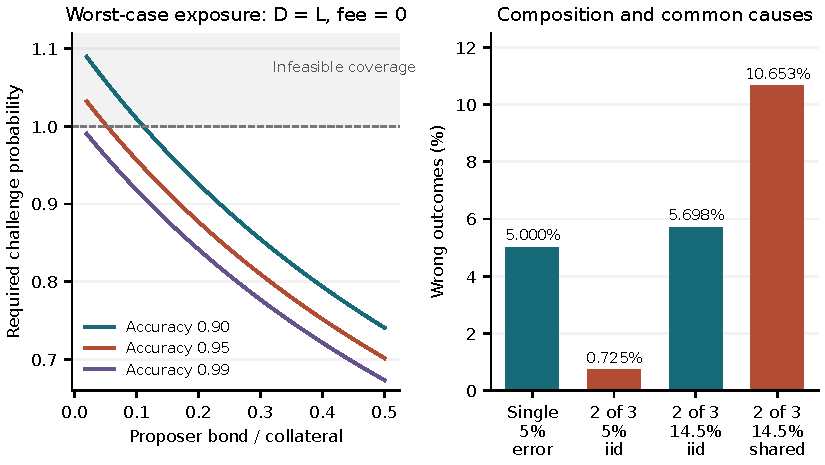
\includegraphics[width=\linewidth]{frontier_and_composition.pdf}
\caption{Exact conditional results. Left: coverage required to deter whole-pool exposure with zero success fee; values above one are infeasible. Right: executed majority-rule error under independent and common-cause input errors. The two rightmost bars match marginal source accuracy.}
\label{fig:frontier_composition}
\end{figure}

\begin{table}[t]
\centering
\caption{Executed source rules with explicit availability endpoints. Rates are exact per offered run. Outage rows use source error 0.05 and either independent 0.20 unavailability per source or a common 0.20 outage. A cancellation is neither a correct Boolean answer nor a deterred economic attack.}
\label{tab:source_results}
\small
\begin{tabularx}{\linewidth}{@{}Yrrr@{}}
\toprule
Source process & Wrong & Correct & Cancel \\
\midrule
Three independent, $e=0.05$ & 0.725\% & 99.275\% & 0\% \\
Matched common error & 10.6525\% & 89.3475\% & 0\% \\
Independent error and outage & 0.4672\% & 85.4848\% & 14.048\% \\
Common outage & 0.580\% & 79.420\% & 20\% \\
One forced corruption & 0\% & 100\% & 0\% \\
Two forced corruptions & 100\% & 0\% & 0\% \\
Two reports withheld & 0\% & 0\% & 100\% \\
\bottomrule
\end{tabularx}
\end{table}

For authority costs $(2,4,6)$, the cheapest two-authority corruption costs 6. Adding a common upstream controlling all reports at cost 3 reduces that minimum to 3, exactly as the authority-cover formula predicts. These are declared cost units. Adaptive budget-constrained attacks also exploit natural errors and outages; one deliberate corruption can join an otherwise honest source error, so the deterministic threshold result is not an unconditional error bound.

The trace tests reinforce the architectural thesis. An executor can fabricate a coherent report and recompute its hash, but fails pinned-source authentication. A genuine source can sign a false statement and pass authentication; an independent dispute remains necessary. Missing or late trace data blocks finalization and follows the explicit timeout rule. Trust becomes visible in the point at which each attack is accepted or rejected.

\section{Interpretation}

The central result is constructive: resolution must be an explicit mechanism whose logic, authority, funding, and failure transitions can be inspected together. The research artifacts execute that mechanism and check its accounting as well as its outcome.

Three results carry the argument. First, sublinear exposure penalties fail when extractable gain scales and correction remains imperfect. Second, costly inspection is a service: a bounty-only equilibrium needs some fraud, while a funded and enforceable work contract can support truthful submission without waiting for errors to finance it. Third, composition raises the cost of producing an accepted wrong input only to the extent that it raises the number or cost of independent authorities an attacker must control.

These results reinforce one another. A trace lowers the cost of finding a precise defect, but someone must still retrieve and check it. A bond changes incentives, but someone must still be able to post a challenge. A quorum raises a source-control threshold, but shared dependencies can collapse it. Trust explicitness is the mechanism that makes these relationships inspectable before participants commit capital.

\section{Protocol Implications and Product Validation}
\label{sec:product}

The analysis yields a concrete design for question.market:
\begin{enumerate}
\item \textbf{Commit the whole constitution.} Pin the question, interpreter, main and dispute programs, source identities, deadlines, cancellation rule, and funding policy before trading. Render the trust profile from those bytes.
\item \textbf{Publish complete, authenticated evidence.} Bind the full trace and enforce publication deadlines. Verify source origin separately from replay consistency. Declare the availability authority or service used to make the gate enforceable.
\item \textbf{Set an exposure and correction target.} Size $B_P+F$ against a conservative $D$ and the effective correction probability $aq$. Treat a binding bond cap or increased external exposure as a change to that guarantee.
\item \textbf{Fund both sides of resolution.} Pay for valid proposal work, including a valid cancellation; reserve funds before accepting the service obligation. Pay for routine inspection when rare fraud cannot sustain coverage, and enforce the checking work under an explicit audit contract.
\item \textbf{Preserve challenge capital.} Work stakes, challenge bonds, concurrent markets, and lock periods draw on the same liquid capital. Measure effective capacity after those commitments, not the count of registered verifier addresses.
\item \textbf{Derive the window from service capacity.} Start usable challenge time only when the evidence is available. Estimate eligible arrival intensity and choose a deadline that meets the coverage target.
\item \textbf{Test correlated failures.} Identify shared source and serving dependencies; test common outages, common wrong reports, unauthenticated fabrication, and strategic withholding.
\end{enumerate}

Question.market is well positioned to validate this design because one product can expose the immutable workflow, evidence publication, proposal service, inspection work, and final payouts. The valuable next experiment is an instrumented deployment of that complete chain. A DAG editor or a low observed dispute rate alone cannot validate the economic thesis.

A prospective product study should randomize funded market-level inspection policies within strata of exposure, source class, and expected activity; predeclare sample size, effect size, stopping rule, and primary endpoints; and record independent ground-truth adjudication. In a controlled environment, blinded injected trace faults and source contradictions give an observable denominator for missed errors. They test detection and escalation without exposing real traders to deliberately false settlement. Track evidence availability, time to first valid check and challenge, eligible capital, audits of work, honest false-challenge cost, proposal willingness, and the three final endpoints: correct, wrong, or unresolved/cancelled. Repeated markets sharing the same source or inspector pool must be analyzed as dependent clusters.

Those measurements estimate the quantities in the proofs: $D$, $q$, $a$, $c$, $\delta$, capital availability, and common failure rates. Power comes from market or provider clusters, not from counting many reports from one shared source as independent observations. The present experiments establish mechanism behavior under explicit inputs. The product study can then test whether the inputs required for the desired guarantee can actually be purchased and sustained.

\section{Scope of the Guarantees}
\label{sec:boundaries}

The analytical guarantees are conditional and constructive: each states the budget, information, independence, or audit assumptions under which it follows. The funded economic experiment is a one-shot policy game; the neutral inspection experiment solves a strategic subgame. Neither claims to solve arbitrary collusion, all sequential waiting equilibria, cross-market portfolios, or endogenous source bribery. Externally correlated positions must enter the exposure bound, and compromised adjudication enters $a$ or the declared fallback authority.

The blueprint experiment provides executable semantics, authenticated fixtures, independent replay, and an explicit publication gate. It does not benchmark production network availability, live LLM judgment quality, smart-contract consensus enforcement, or a deployed work-audit technology. A production interpreter can implement the same contract while using a different engine. Deployment divergence does not change the paper's specified mechanism or its reproduced results.

No structural mechanism repairs a semantically incoherent question. The committed question/program pair must define outcome scope, edge cases, evidence policy, and valid cancellation. Making those choices immutable makes their quality inspectable; it does not make a bad choice good. The publication's strength is that each assumption now has a concrete object to inspect, a theorem to apply, or an experiment to run.

\section{Conclusion}

Resolution is where trust concentrates in prediction markets. Pricing, liquidity, order matching, and settlement can be made mechanical. Resolution still requires an external claim about what happened in the world. The question is whether that claim arrives through a process the participant can inspect and hold to account.

Trust-explicit resolution gives each market an executable constitution. The program fixes how evidence is obtained, how judgment enters, which branches can settle or cancel, and how a challenge is decided. Canonical full-trace commitments bind the reported execution; source authentication identifies its authorities; an availability gate makes checking possible. The trust profile exposes what each of those checks can establish.

The economic requirements are equally concrete. Bonds must track extractable exposure when correction remains imperfect. Thin-market integrity is constrained by actual checking. Open service needs compensation, and paying for verification works only when verifying beats shirking and enough challenge capital remains. Independent source composition raises the corruption threshold; common dependencies lower it. Proofs, 855{,}000 funded-game episodes, exact inspection equilibria checked by 900{,}000 further episodes, and executed corruption tests support those claims.

Trust-explicit resolution does not eliminate trust. It makes trust visible, bounded, and challengeable. A market should carry its own executable resolution constitution, and the protocol should fund the people and processes that make that constitution binding.

\appendix

\section{Executable Profile and Reproduction Contract}
\label{app:semantics}

The reference package exposes three independent entry points:
\begin{quote}\small\ttfamily
python -m research.resolution\_trust.economy\_validation\\
python -m research.resolution\_trust.monitoring\_game\\
python -m research.resolution\_trust.blueprint\_experiments
\end{quote}
Each accepts an explicit output directory. The public reproduction guide records complete commands, environment requirements, hashes, and figure generation. The Boolean profile's normative schema and test-vector identifiers are supplied in \texttt{BLUEPRINT\_PROTOCOL.md}; the mathematical rules needed to interpret the results are specified in this paper.

For a Boolean run, report nodes are sorted by identifier and terminals join all distinct reports. Reports carry signed scope (blueprint, event, market, run, node, authority, request, observation time, and Boolean value). Only authenticated source publications may occupy their source slot. The first admitted publication is binding. The checker reconstructs every expected report record and all terminal records, including skipped terminals, and rejects differences rather than trusting proposer-supplied output summaries. The mutually exclusive guards are: a strict-majority quorum submits; no quorum with remaining run budget defers; no quorum on the final run cancels.

A successor run starts at the fixed previous start plus retry delay and binds its predecessor root. It is permitted only after defer. At the hard deadline
\[
t_{\rm hard}=t_{\rm initial}+(N_{\rm runs}-1)\,\Delta_{\rm retry}
              +W_{\rm source}+W_{\rm publication}+1,
\]
unresolved state becomes \texttt{cancel\_timeout}. Accepted Boolean results and cancellations cannot reopen. The clock and append-only publication service are explicit trusted inputs to these transitions.

The main economics grid saves every episode in compressed JSON Lines. The monitoring suite saves all equilibria, three-seed Monte Carlo summaries, and deterministic samples, with seeds sufficient to regenerate all episodes. The source suite saves all canonical trace vectors and every weighted state; its 14 verification vectors include two accepted controls and 12 intentionally invalid cases, all blocked. Paper figures are regenerated from these current artifacts. Historical aggregate files have no evidentiary role in the revised quantitative claims.

\section{Claim-to-Evidence Map}

\begin{longtable}{@{}p{0.39\linewidth}p{0.54\linewidth}@{}}
\toprule
Claim & Evidence \\
\midrule
\endfirsthead
\toprule Claim & Evidence \\
\midrule
\endhead
An immutable program and full trace bind the declared procedure and reported run & Proposition~\ref{prop:binding}; independent replay; tamper, scope, authentication and availability vectors. \\
Flat exposure penalties fail at scale & Theorem~\ref{thm:deterrence}, Corollary~\ref{cor:scaling}; funded bond and cap sweeps with separate submission endpoints. \\
Coverage is the low-attention bottleneck & Exact decomposition~\eqref{eq:failure_decomposition}; paired attention, window, and adjudication experiments. \\
Routine checking needs an incentive-compatible service contract & Propositions~\ref{prop:rare_fraud} and~\ref{prop:paid_inspection}; exact verify/shirk/idle equilibria, unaudited control, fresh capital/outage regimes. \\
Proposer fees support truthful service & Participation inequality; compensation sweeps; no-fee/no-proposal controls. \\
Independent source composition raises corruption cost & Proposition~\ref{prop:source_cost}; 30 executed source-state vectors; exact authority-budget search and matched common-error control. \\
Question.market can validate the required operational inputs & Prospective protocol in Section~\ref{sec:product}; a product study remains to be executed. \\
\bottomrule
\end{longtable}

\section*{Author Note}

This manuscript was developed with large language model assistance for simulation architecture design, mathematical formalization, literature review, and critical review of drafts. The underlying mechanism design, economic thesis, implementation choices, calibration objectives, and earlier prototypes are the author's own.

\begin{thebibliography}{99}

\bibitem{hanson2002}
Robin Hanson.
\newblock \emph{Logarithmic Market Scoring Rules for Modular Combinatorial Information Aggregation}.
\newblock Working paper, 2002.
\newblock Available at \url{https://mason.gmu.edu/~rhanson/mktscore.pdf}.

\bibitem{uma2021}
UMA Protocol.
\newblock \emph{Optimistic Oracle}.
\newblock Documentation, accessed 2026.
\newblock \url{https://docs.uma.xyz/protocol-overview/how-does-umas-oracle-work}.

\bibitem{realityeth}
Edmund Edgar.
\newblock \emph{Reality.eth: a crowd-sourced on-chain oracle}.
\newblock Documentation, accessed 2026.
\newblock \url{https://reality.eth.limo/}.

\bibitem{kleros2019}
Federico Ast and Cl\'{e}ment Lesaege.
\newblock \emph{Kleros: Short Paper}.
\newblock Working paper, 2019.
\newblock Available at \url{https://kleros.io/whitepaper.pdf}.

\bibitem{polymarket2024}
Polymarket.
\newblock \emph{How Resolution Works}.
\newblock Documentation, accessed 2026.
\newblock \url{https://help.polymarket.com/en/articles/13364518-how-are-prediction-markets-resolved}.

\bibitem{augurv2}
Augur.
\newblock \emph{Augur v2 Whitepaper}.
\newblock 2019.
\newblock \url{https://github.com/AugurProject/whitepaper}.

\bibitem{gnosisct2026}
Gnosis.
\newblock \emph{Conditional Tokens Developer Guide}.
\newblock Documentation, accessed 2026.
\newblock \url{https://conditional-tokens.readthedocs.io/en/latest/developer-guide.html}.

\bibitem{metaculus2026}
Metaculus.
\newblock \emph{Question Writing and Resolution Guidelines}.
\newblock Documentation, accessed 2026.
\newblock \url{https://www.metaculus.com/help/prediction-resources/}.

\bibitem{buterin2014}
Vitalik Buterin.
\newblock \emph{SchellingCoin: A Minimal-Trust Universal Data Feed}.
\newblock Blog post, 2014.
\newblock \url{https://blog.ethereum.org/2014/03/28/schellingcoin-a-minimal-trust-universal-data-feed}.

\bibitem{umamoop2025}
UMA Protocol.
\newblock \emph{Improving Oracle Efficiency with Managed Proposers}.
\newblock UMA blog, August 2025.
\newblock \url{https://blog.uma.xyz/articles/managed-proposers}.

\bibitem{sztorc2015}
Paul Sztorc.
\newblock \emph{Truthcoin: Peer-to-Peer Oracle System and Prediction Marketplace}.
\newblock Working paper, 2015.
\newblock \url{https://bitcoinhivemind.com/papers/truthcoin-whitepaper.pdf}.

\bibitem{chainlink2017}
Steve Ellis, Ari Juels, and Sergey Nazarov.
\newblock \emph{ChainLink: A Decentralized Oracle Network}.
\newblock White paper, 2017.
\newblock \url{https://research.chain.link/whitepaper-v1.pdf}.

\bibitem{eskandari2021}
Shayan Eskandari, Mehdi Salehi, Wanyun~Catherine Gu, and Jeremy Clark.
\newblock \emph{SoK: Oracles from the Ground Truth to Market Manipulation}.
\newblock In \emph{Proceedings of the 3rd ACM Conference on Advances in Financial Technologies (AFT '21)}, 2021.

\bibitem{daian2019}
Philip Daian, Steven Goldfeder, Tyler Kell, Yunqi Li, Xueyuan Zhao, Iddo Bentov, Lorenz Breidenbach, and Ari Juels.
\newblock \emph{Flash Boys 2.0: Frontrunning, Transaction Reordering, and Consensus Instability in Decentralized Exchanges}.
\newblock In \emph{Proceedings of the 2020 IEEE Symposium on Security and Privacy}, pages 910--927, 2020.

\bibitem{teutsch2019}
Jason Teutsch and Christian Reitwie{\ss}ner.
\newblock \emph{A Scalable Verification Solution for Blockchains}.
\newblock Technical report, 2019.
\newblock \url{https://people.cs.uchicago.edu/~teutsch/papers/truebit.pdf}.

\bibitem{witnet2026}
Witnet.
\newblock \emph{HTTP GET Requests in Solidity}.
\newblock Oracle documentation, accessed October 2026.
\newblock \url{https://docs.witnet.io/smart-contracts/witnet-web-oracle/make-a-get-request}.

\bibitem{koch2018}
Julia Koch and Christian Reitwie\ss ner.
\newblock \emph{A Predictable Incentive Mechanism for TrueBit}.
\newblock arXiv:1806.11476, 2018.
\newblock \url{https://arxiv.org/abs/1806.11476}.

\end{thebibliography}

\end{document}
